\documentclass[12pt]{article}

\usepackage[german]{babel}
\usepackage{amsmath}
\usepackage{amssymb} % to display symbols for real numbers, integers etc. Usage: \mathbb{R}
\usepackage{graphicx}
\usepackage{listings} % to display programming code
%\usepackage[ngerman]{babel}
\usepackage{color}
\usepackage{relsize} % to display scaled math symbols (big summation symbol etc.)
\usepackage{textcomp}

\DeclareGraphicsExtensions{.pdf,.jpeg,.png}
\definecolor{listinggray}{gray}{0.9}
\definecolor{lbcolor}{rgb}{0.9,0.9,0.9}
\lstset{ % to display programming code in nice colors
	backgroundcolor=\color{lbcolor},
	tabsize=4,
	rulecolor=,
	language=matlab,
		basicstyle=\scriptsize, %for extra small font size
        upquote=true,
        aboveskip={1.5\baselineskip},
        columns=fixed,
        showstringspaces=false,
        extendedchars=true,
        breaklines=true,
        prebreak = \raisebox{0ex}[0ex][0ex]{\ensuremath{\hookleftarrow}},
		frame=single, %draw frame
        showtabs=false,
        showspaces=false,
        showstringspaces=false,
        identifierstyle=\ttfamily,
        keywordstyle=\color[rgb]{0,0,1},
        commentstyle=\color[rgb]{0.133,0.545,0.133},
        stringstyle=\color[rgb]{0.627,0.126,0.941},
        numbers=left,
        stepnumber=1,
        firstnumber=1,
        numberfirstline=true,
        linewidth=14cm,
}

\title{\"Ubungsblatt 7\\ \glqq Mustererkennung\grqq}
\author{J. Cavojska, N. Lehmann, R. Toudic}
\date{16.06.2015}
\begin{document}
\maketitle
%\renewcommand{\contentsname}{Table of Contents}
\tableofcontents
\newpage

\section{Logistische Regression}

\subsection{Code}

\begin{lstlisting}[language=Matlab]
% Clean up
clear all
close all
clc

% Datenaufbereitung
Data         = load('fieldgoal.txt');
ExtendedData = [Data(:,1), ones(size(Data,1), 1)];
Distance     = Data(:,1);
Goal         = Data(:,2);
N            = length(Data);
limit        = 100000;
x_range        = linspace(0,100);
x_print        = [0:100];

%%% Aufgabe 1 - Logistische Regression %%%

figure('NumberTitle','off','Name','Aufgabe 1 - Logistische Regression');

alpha = 10e-7;
beta  = [0;0];   % initiales beta

for i = 1:limit
    
    t = beta' * ExtendedData';
    p = exp(t')./(1.+exp(t'));
    
    likelihood = ExtendedData' * ( Goal - p );

    beta = beta + (alpha * likelihood);
    
    if mod(i,25000) == 0
        
        % Fehler berechnen
        e = sum(abs(Goal - p))
        
        % Wahrscheinlichkeit für einen Treffer berechnen
        p_estimate = 1./(1.+exp(-(beta(2)+ beta(1)*x_print)));
        
        % plot
        hold off
        scatter(Distance, Goal);
        hold on
        plot(x_print,p_estimate,'r');
        
        title('Aufgabe 1 - Logistische Regression');
        xlabel('Distanz zum Tor');
        ylabel('Wahrscheinlichkeit für einen Treffer')
        axis([-0.1 100.1 -0.1 1.1]);
        legend('Datenpunkte','p(x,beta)');
        
        pause(0.0001) % gib Matlab Zeit zu plotten!
    end
end

% error-output
% 329.2452
% 313.5010
% 302.3904
% 294.3464
\end{lstlisting}

\newpage

\subsection{Bilder}

\begin{center}
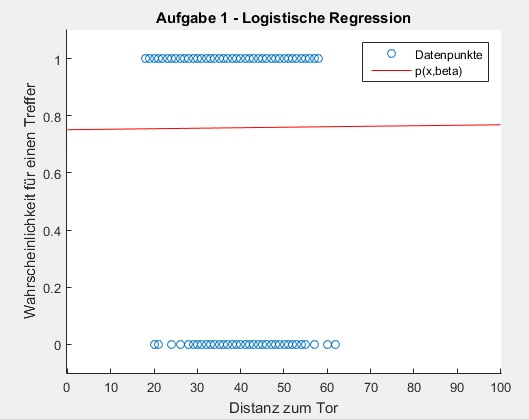
\includegraphics[width=10cm]{plot1.jpg}
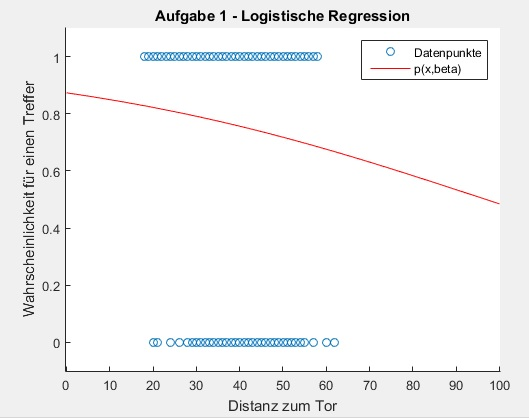
\includegraphics[width=10cm]{plot2.jpg}
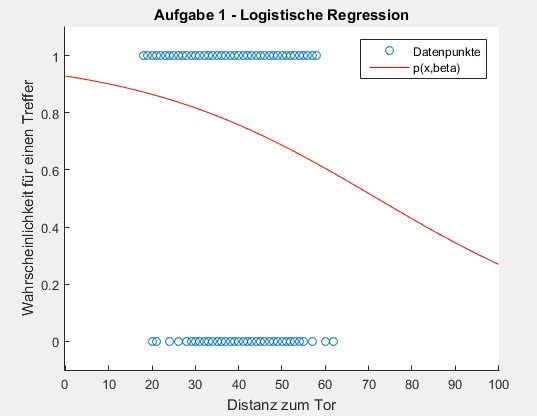
\includegraphics[width=10cm]{plot3.jpg}
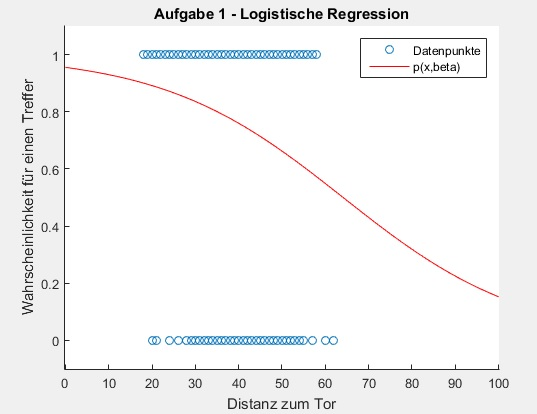
\includegraphics[width=10cm]{plot4.jpg}
\end{center}


\end{document}